\chapter{Background}
\label{chap:background}

\section{Medical Background}
This section introduces the reader to the dementia disease, some of its symptoms and explain why it is not a normal stage of life. 

\label{sec:medical_background}

\subsection{Dementia}
Dementia is not a specific disease but an overall term used to group all diseases that are characterized by a decrease in memory, thinking capabilities, language and other skills related to the thought. With between 60 and 70 percents\footnote{\href{https://www.who.int/news-room/fact-sheets/detail/dementia}{https://www.who.int/news-room/fact-sheets/detail/dementia}} of the cases, Alzheimer's Disease (AD) is the most common disease-causing dementia. Despite the fact that dementia is affecting mostly old people, it is not a normal stage of life and therefore should not be seen as severe ageing.

\begin{figure}
 \centering
 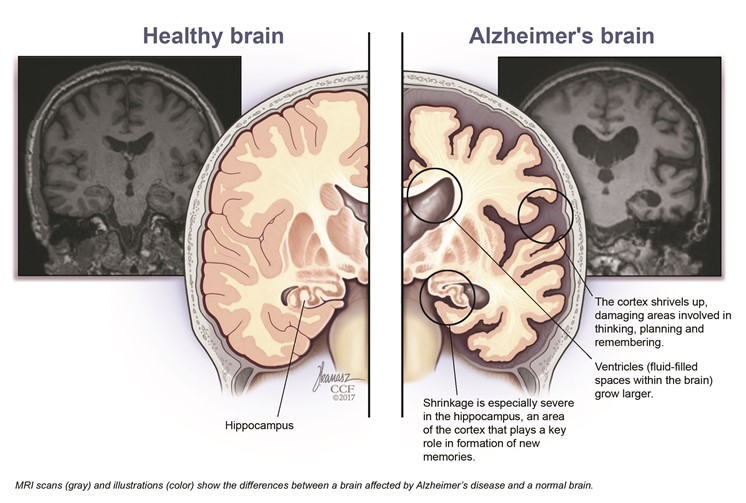
\includegraphics[width=400]{figures/Alzheimer_brain.jpg}
 \caption[Test]{Illustration\footnotemark of the differences between a healthy brain and the brain of someone with Alzheimer disease.}
 \label{fig:alzheimerbrain}
\end{figure}
\footnotetext{\href{https://www.keepmemoryalive.org/brain-science/alzheimers-brain}{https://www.keepmemoryalive.org/brain-science/alzheimers-brain}}

Figure~\ref{fig:alzheimerbrain} highlights the visual differences that practitioners can use to diagnose a Alzheimer patient. Knowing which part of the brain is affected by the disease will help us evaluate our model. We expect a good model to focus his attention on these brain areas in order to make its prediction. In fact, one would more easily trust a model that has the same attention locations as a clinician, in agreement with the medical knowledge.

\subsection{Current Methods}
Most current methods in dementia research are based on the on comparing MRI scans from healthy participants to the scans from patients with dementia. this required that all the brain scans are aligned to a common template, as describe in section~\ref{sec:coregistration}. The goal is that a voxel at a specific coordinate is mapping to the same brain location on both images. This also allows to remove the large differences of brain anatomy between subjects. For completeness of the study, we performed this method called Voxel-Based Morphometry\cite{voxel_based_morphometry_ASHBURNER2000805} in annex~\ref{chap:Morphometry_analysis}.

Some classical machine learning\cite{classical_ml_methods_SAMPERGONZALEZ2018504} approach such as SVM\cite{svm_article}, logistic regression and Random Forest\cite{random_forest_10.1023/A:1010933404324} have been use to detect dementia. These methods require the data to be heavily preprocessed.


\subsection{Age vs. Dementia}

It is tempting to see dementia damaged brain as an extreme ageing process. In both cases, we observe a loss of white matter due to neuron death. Even though scientists currently do not know exactly what causes the disease, they do observe the presence of biomarkers such as plaque and tangle \cite{alzheimer_past_present_future}.

Despite the differences, researcher\cite{brain_age_10.3389/fneur.2019.00789} have built simple dementia detectors by training an age predictor on healthy brains. It appears that their predictor performs badly on dementia's brains and tends to overage people with the disease. As we trained an age predictor on healthy brains, in annex~\ref{chap:age_pred} we took the opportunity to try it on our data. In fact, as shown in the annex, it turns that our predictor is not able to distinguish between healthy and sick brains as it can be seen in figure~\ref{fig:dem_vs_control_age_pred}. This tends to show that indeed the assumption is wrong and that the people with dementia do not have an overaged brain.

In general, it would be more interesting to build a model that is able to detect dementia regardless of the patient's age, therefore reducing as much as possible the bias of the model towards age.


\section{Model Blocks}
This section defines fully connected and convolutional layers which are the two machine learning blocks that we are using in this project.
\subsection{Fully Connected}

One of the most basic components when building a deep learning model is the fully connected (FC) layer. Mathematically it is defined as:
$$Y=X*W + b$$
Where the outputs $Y$ are expressed as a linear combination of the inputs $X$ using a weight matrix $W$ and a bias $b$. It has been proven by the well-known \textit{universal approximation theorem}\cite{universal_approx_theorem_10.5555/70405.70408} that such layers combine with non-linear functions can approximate in theory any continuous functions.

\subsection{Convolutional Neural Networks}

The fully connected layer presented above is really general and works well with a large variety of data. Unfortunately, for certain types of data, using FC layers can quickly become unscalable. For example, when dealing with images of size 200 by 200 in color (RGB), a layer with 100 features output would already require 12'000'100 parameters to be learned (including bias). 

Convolutional Networks\cite{cnn_original_paper_10.5555/646469.691875} were introduced by LeCun to minimize the processing done on the input image and let the network learn the right set of features. For it to be working, convolutional layers have to make assumptions on the data. One is spatial locality, where the pixels close to each other are more likely to be correlated than distant ones. In fact, CNN can be seen as small FC layers that are applied at multiple locations across the image. These are usually called kernels. The assumptions made by CNN reduce the number of parameter of the network. This helps for regularization and the network requires less data to be train.


This way of computing the inputs does have multiple advantages, one of them being weight-sharing. The kernel being applied at multiple locations, the weights learned to extract a feature in one location are by construction reused to extract the same features everywhere else in the image. Another property of CNN that comes directly from their formulation is the fact that translating the input, results in a translated output, this is called translation equivariance. Nowadays, CNN has become the standard way of processing images.
\begin{wrapfigure}{r}{0.6\textwidth}
 \centering
 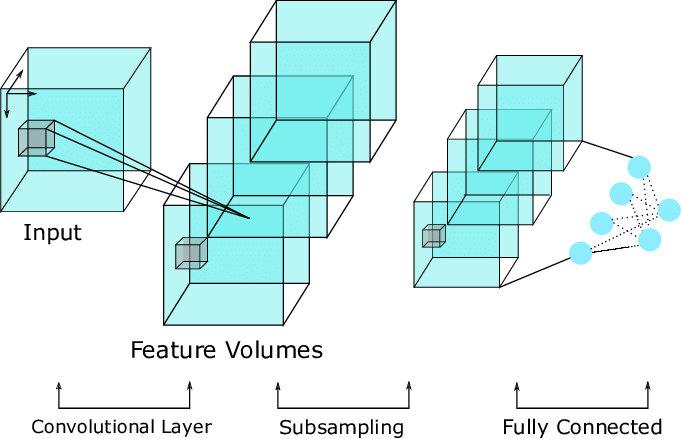
\includegraphics[width=.9\linewidth]{figures/3D_CNN_example.png}
 \captionsetup{width=.9\linewidth}
 \caption[3D_CNN_example]{Illustration\footnotemark{} of a 3D CNN}
 \label{fig:3d_cnn_example}
\end{wrapfigure}
\footnotetext{\href{https://www.researchgate.net/publication/330912338_ECNN_Activity_Recognition_Using_Ensembled_Convolutional_Neural_Networks}{https://www.researchgate.net/publication/330912338\_ECNN\_Activity\_Recognition\_Using\_Ensembled\_Convolutional\_Neural\_Networks}}


In our case, we are dealing with 3D images (MRI) that are scientifically larger than standard 2D ones, therefore it makes even more efficient to use 3D convolutions. As illustrated by figure~\ref{fig:3d_cnn_example}, 3D CNN are really similar to 2D CNN. The only difference between 2D CNN and 3D CNN is the shape of the learned kernels, which are three-dimensional in order to fit the input.


\section{Losses and Metrics}
\label{sec:losses_metrics}
This section lists the different metrics, and losses used during this project.

\subsection{Binary Cross Entropy}
\label{sec:binary_cross_entropy}
This loss is used to measure the error made on binary classification.
$$ L = -(y\log(p) + (1-y)\log(1-p))$$
Where $p$ is the predicted probability of belonging to the class made by network and $y$ the binarized true label. 

\subsection{Mean Square Error (MSE)}
\label{sec:mean_square_error}
This loss is used to penalize errors made by a network for example in the case of a regression. It works with continuous values and is defined as:
$$ MSE = \frac{\sum_{i=1}^{n} (Y_i - \^{Y}_i)^2}{n}$$

Where $\^{Y}_i$ is the predicted value and $Y_i$ is the target value, $n$ is the total number of samples and $i$ the running index of a sample in the summation.
\subsection{Mean Absolute Error (MAE)}
This metric is really similar to the MSE, but we take the absolute value of the error instead of taking the square.
$$ MAE = \frac{\sum_{i=1}^{n} |(Y_i - \^{Y}_i)|}{n}$$

Where $\^{Y}_i$ is the predicted value and $Y_i$ is the target value, $n$ is the total number of samples and $i$ the running index of a sample in the summation.
\subsection{Accuracy}
The accuracy is one of the simplest metrics to evaluate a model. It is computed by counting the number of correctly classified samples divided by the total number of samples.


\subsection{Precision and Recall}
While accuracy is simple to understand and to visualize, it can often fail at evaluating the performance of a model when the dataset has unbalanced classes. To overcome this issue other metrics can be computed based on the true/false positive and true/false negative.

\begin{itemize}
    \item \textbf{True positive (TP)}: Positive sample correctly classified as positive. 
    \item \textbf{False positive (FP)}: Negative sample badly classified as positive. 
    \item \textbf{True negative (TN)}: Negative sample correctly classified as negative. 
    \item \textbf{False negative (FN)}: Positive sample badly classified as negative.
\end{itemize}

Precision can thus be computed as below and gives a sense of how precise the classifier is on dementia predicted brains.
$$Precision = \frac{TP}{TP +  FP}$$

Recall on the other hands can be computed as below and gives a sense of how likely the model is to detect dementia when the patient is indeed ill.
$$Recall =\frac{TP}{TP + FN}$$
In a medical situation, it might be more interesting to have a model with a good recall at the expense of precision, namely having more false positive. The consequences of being detected as healthy when in fact the patient suffers from the disease are often worse than the opposite.

Accuracy can also be computed with these terms.


$$Accuracy = \frac{TP + TN}{TP + TN + FP + FN}$$


\subsection{ROC - AUC}
Receiver Operating Characteristic allows for plotting a chart like figure~\ref{fig:roc_curve} that visualizes the true positive rate against the false positive rate at different thresholds. From this curve, we can compute the Area Under the Curve (AUC) which is a good metric to compare different models. Usually, a bigger AUC means a better model, the rise of the curve is even more important.
In an ideal situation, we expect the curve to touch the top left corner and have an AUC of 1.

\subsection{PR - Curve}
The Precision and Recall curve is often used in replacement of the ROC curve when dealing with unbalanced data. It plots the precision and recalls of the model is computed at different thresholds. An example of PR curve can be seen in figure~\ref{fig:pr_curve}.

\section{Model Explanation}
\label{sec:model_explaination}
There exist multiple ways to explain the output of a model. We tried different approaches that are either specific to computer vision tasks or more general and compared them for our specific task of dementia prediction.

\subsection{Shap}
Shap is an algorithm based on Game Theory that aims to predict the contribution of a feature to increase the confidence of a model. Its mathematical background lies on the Shapley value which basically is the average of the marginal contributions across all permutations of features. Figure~\ref{fig:shap_example} shows what the outcome of the shap algorithm look link on image data.

\begin{figure}
 \centering
 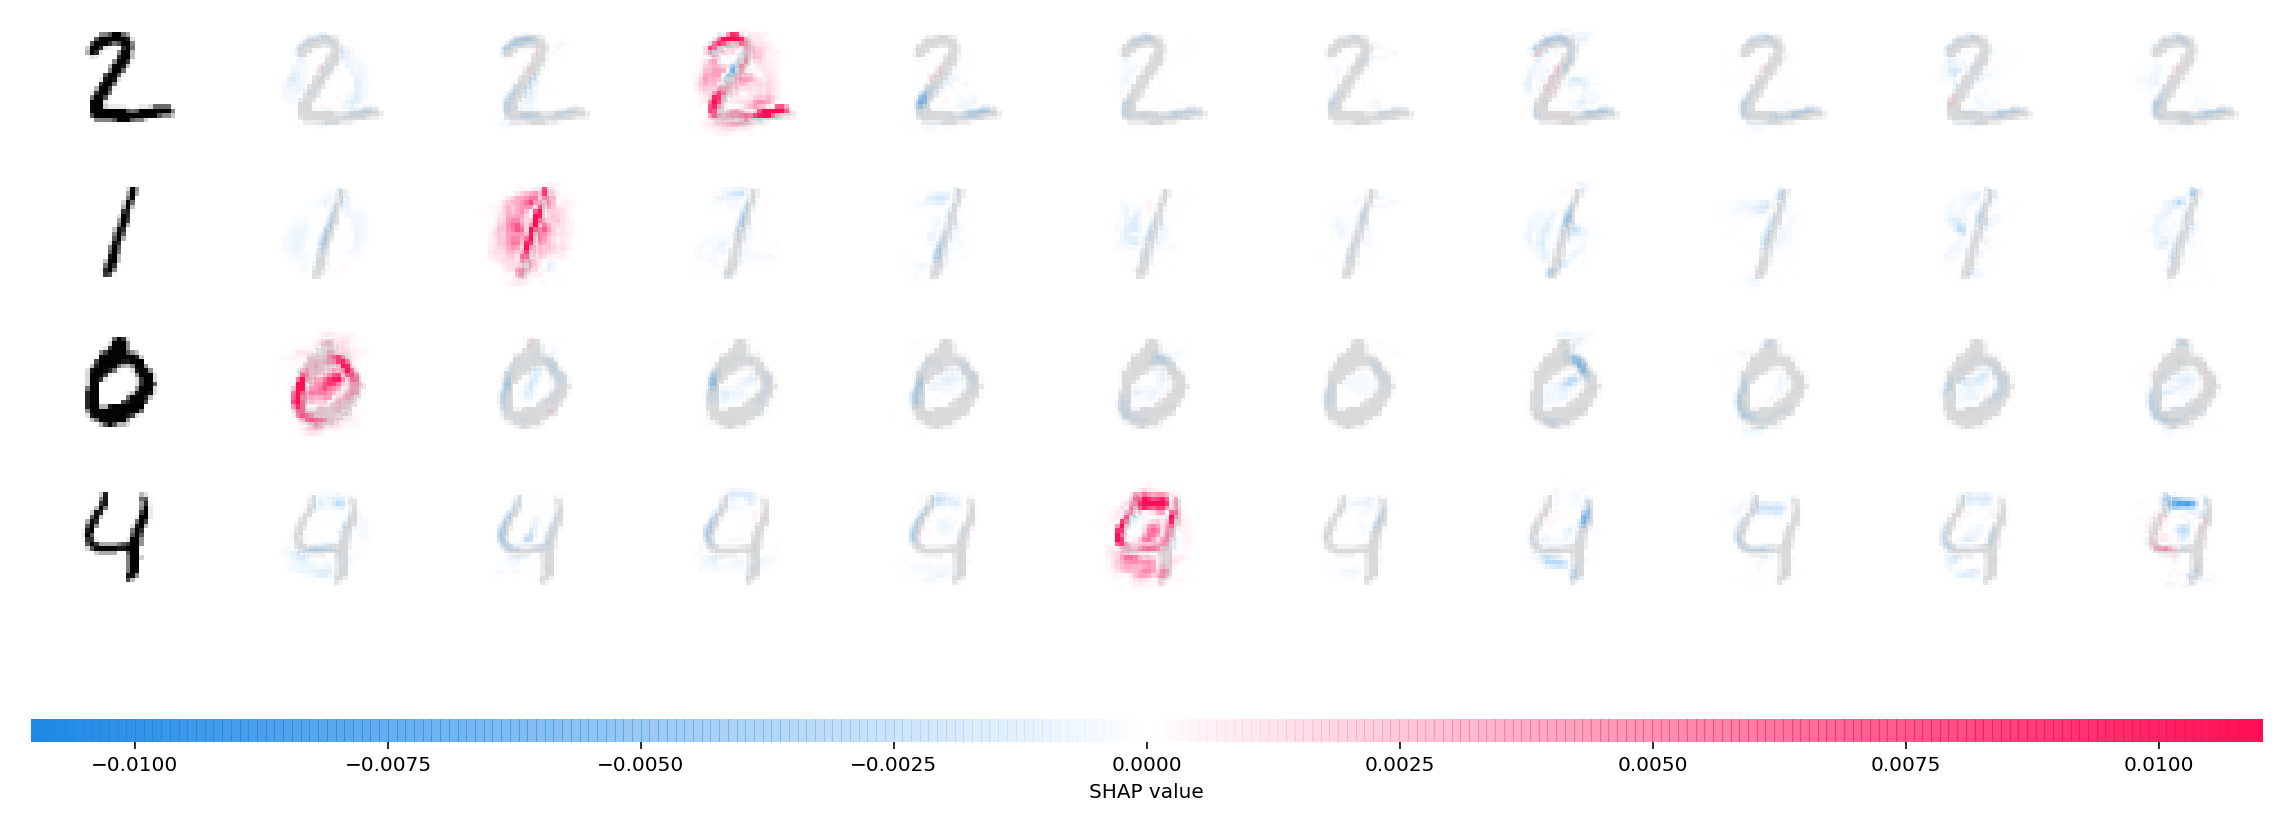
\includegraphics[width=.9\linewidth]{figures/shap_mnist_image_plot.png}
 \captionsetup{width=.9\linewidth}
 \caption[ShapExample]{Example of shap value from the Shap repo\footnotemark{}. Each column represents the shap output for a specific class (in a sorted order).}
 \label{fig:shap_example}
\end{figure}
\footnotetext{\href{https://github.com/slundberg/shap}{https://github.com/slundberg/shap}}

The library\cite{shap_lundberg2017unified} works with different kinds of models but it was tested with the GradientExplainer as DeepExplainer is not fully compatible with Pytorch yet. Compared to some other explainer algorithm, Shap presents the advantage of giving a negative value for a feature which has a negative correlation with the output. The output obtained by this process can be seen in figure~\ref{fig:explainer_compared}, but we can see that it does not give a good interpretation in comparison with other techniques.



\subsection{Grad-Cam}
When the input is an image, analysts are interested in finding out which part of the image better explains the prediction. In his paper\cite{zhou2015cnnlocalization} Zhou, proposes a specific model for which he could create a \textit{class activation maps}. This idea has been generalized to work with any model by the authors of grad-cam. 

\begin{figure}
    \centering
    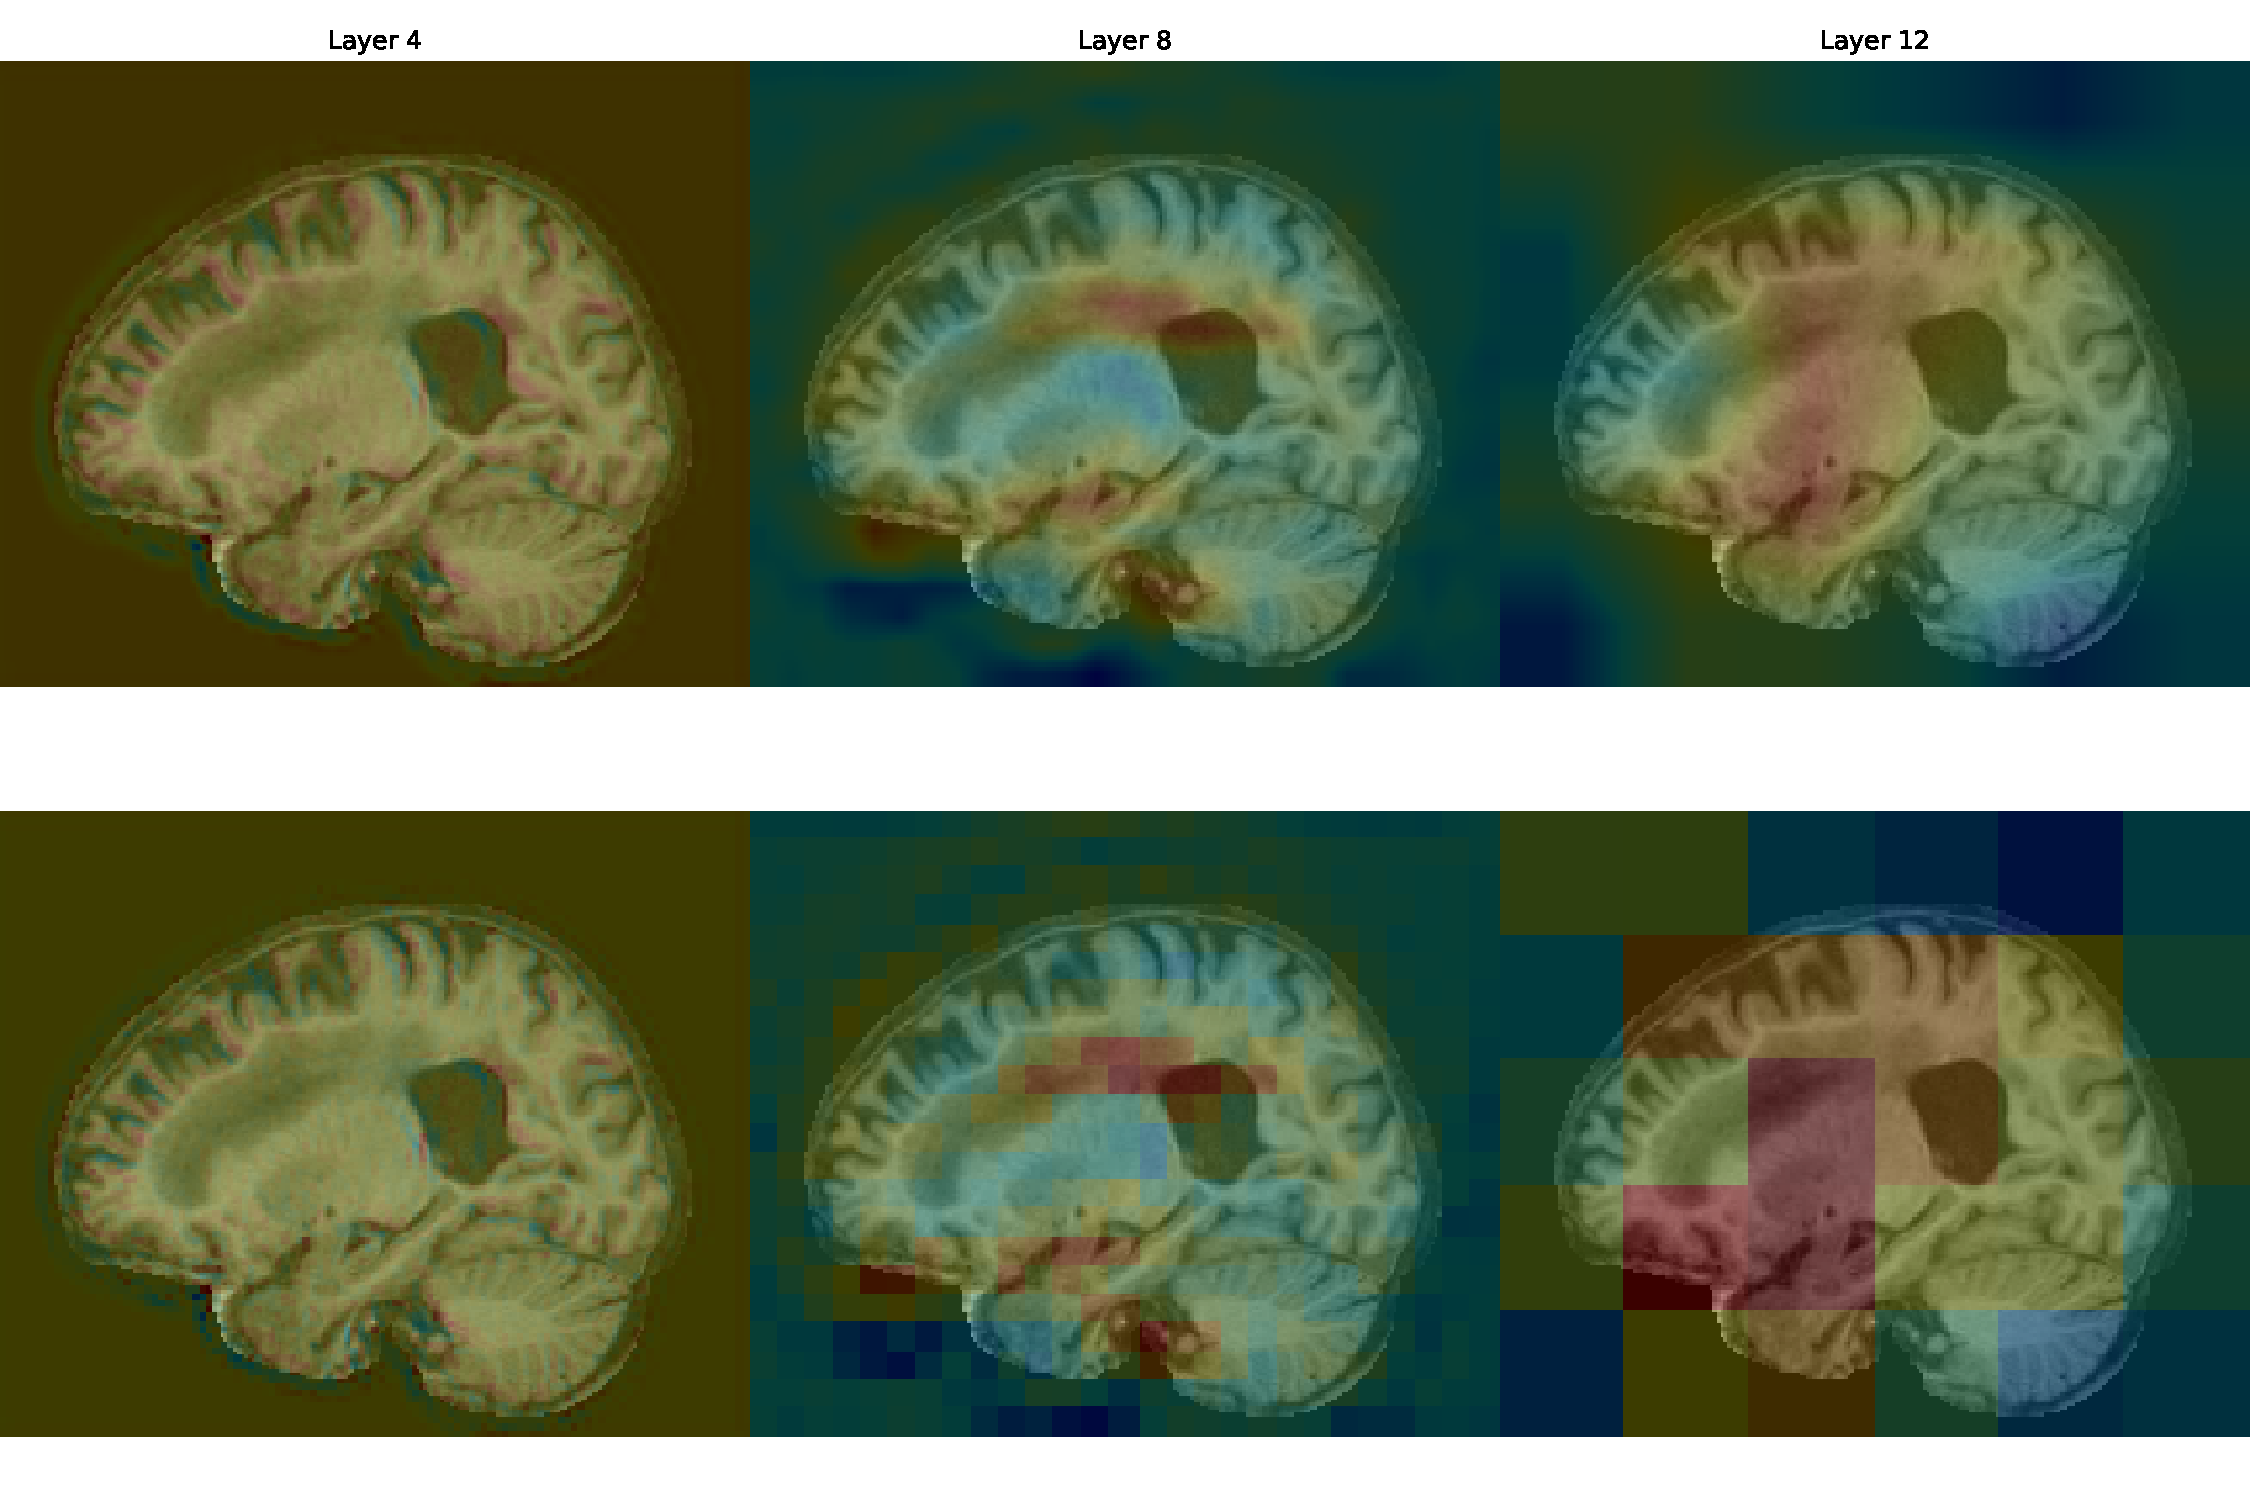
\includegraphics[width=400]{figures/gradcam_multilayer.pdf}
    \caption{GradCam saliency map seen at different layers. Trilinear interpolation is used in the first row and nearest interpolation in the second one.}
    \label{fig:grad_cam_multilayer}
\end{figure}

The Grad-Cam\cite{grad_cam_2019} algorithm is looking for activation of the neurons at a specific layer. To do so the input is processed in a forward pass by the network until the final prediction is made. The gradient of the predicted class with respect to the layer of interest is then computed. It is then pooled across its spatial dimension in order to get a value of layer importance per channel. The features extracted from the image are then multiplied channel-wise by the pooled gradient in order to get an activation map (also called saliency map) of the same shape at the output of the layer of interest. This can be mapped to the original image shape by interpolation. For visual purposes, we choose to do a trilinear interpolation, which is the extension of the bilinear interpolation in three dimensions. A visual comparison of the outcome can be seen in figure~\ref{fig:grad_cam_multilayer}. This algorithm is well schematized in figure~\ref{fig:grad_cam_arch}.

\begin{figure}
    \centering
    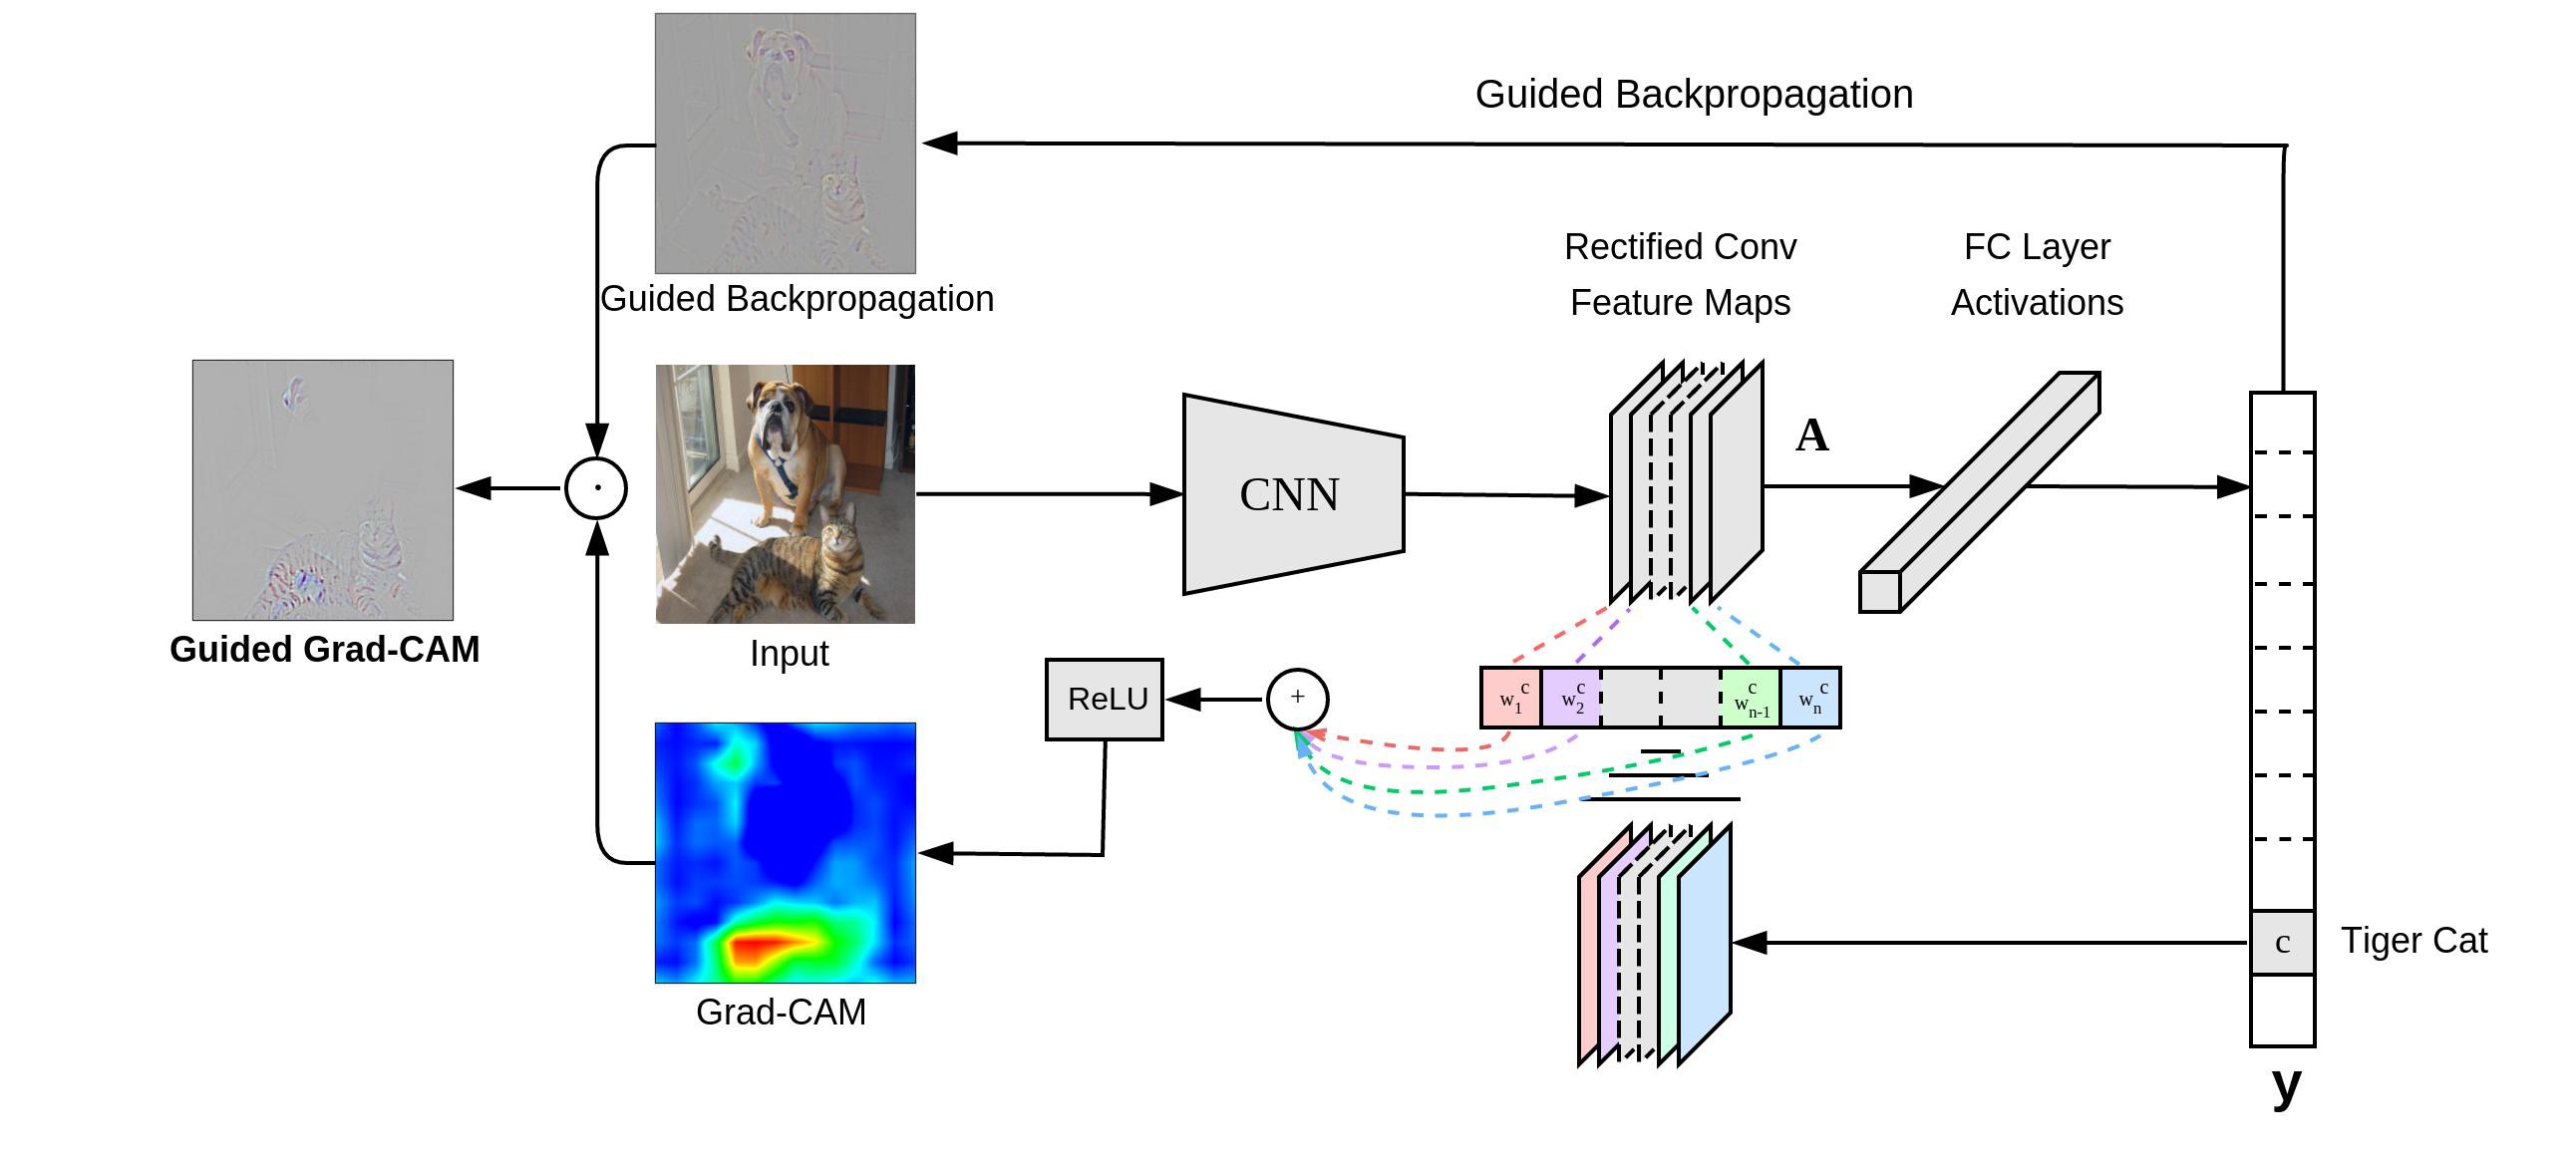
\includegraphics[width=400]{figures/grad_cam_arch.jpeg}
    \caption{Schema of the GradCam algorithm taken from the paper\cite{grad_cam_2019}}
    \label{fig:grad_cam_arch}
\end{figure}

When the model goal is to perform multi-class classification, it makes sense to apply a Relu function to the activation map in order to remove the negative value that could be explaining any other classes in the image. In our case, as we are dealing with a binary classification task, it might make sense not to remove negative values and let a clinician decides which map is more useful for him.

The output size of the layer one tries to explain will determine the granularity of the activation map. The artifact due to shrinkage of the network can be seen in figure~\ref{fig:grad_cam_multilayer}. This imposes a trade-off when constructing the model, either last convolution layer output is too small in order to keep a good focused explanation or it is too big but this induces a bigger model which then needs more data to be trained.

Guided backpropagation\cite{guided_backprop_springenberg2014striving} is another visualization to explain what a model has learned. Compared to grad-cam it gives a sharper explanation map but fails at giving an explanation for a specific class. To get the best of both, it is possible to multiply pointwise the two outputs as illustrated on the left side of figure~\ref{fig:grad_cam_arch}.


\subsection{FullGrad}
\label{sec:fullgrad}

Developed by Sriniva and Fleuret at EPFL, FullGrad\cite{fullgradient} introduce a new tool for neural network interpretability that satisfies both \textit{completeness} and \textit{weak dependence on inputs}. Completeness can be seen as the property that the saliency map contains all the information necessary to compute the output of the model.

\begin{figure}
    \centering
    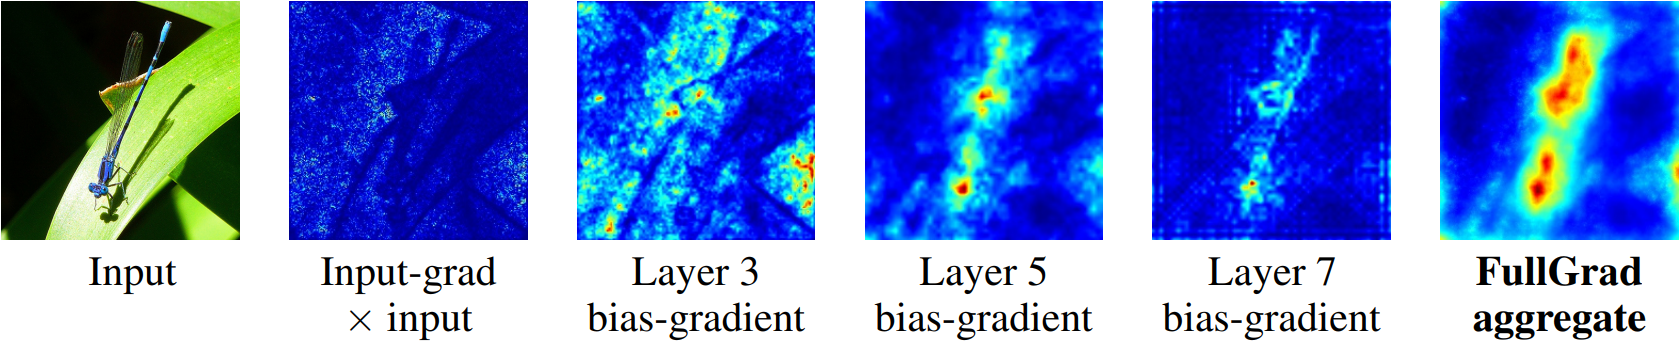
\includegraphics[width=400]{figures/fullgrad_layer_agregation.png}
    \caption[FullGradExample]{Visualization\cite{fullgradient} of bias gradient at different layers and the output of fullGrad which is an aggregation of the input gradient and all the intermediate layers.}
    \label{fig:full_grad_layer_aggreagtion}
\end{figure}

A saliency map is complete if there exists a function $\phi$ such that:

$$\phi(S(x), x) = f(x) \hspace{10} \forall x,f$$

Weak dependence on inputs, on the other hand, is a property that one gets when slightly changing an important pixel drastically affects the output of the model. Previous methods were not able to have these two properties at the same time.

As visualized in figure~\ref{fig:full_grad_layer_aggreagtion} the output of the fullGrad algorithm is an aggregation of the gradient at multiple layers. Therefore, compared to GradCam there is no need to define a layer of interest which is usually set to the last convolutional layer. This also makes the algorithm less sensitive to the potentially small size of the last convolutional layer.